\documentclass[11pt]{beamer}
\usepackage[english]{babel}
\usetheme{Boadilla}
\usepackage[utf8]{inputenc}
\usepackage{amsmath}
\usepackage{amsfonts}
\usepackage{amssymb}
\usepackage{graphicx}
\usepackage{url}
\usepackage{booktabs}
\usepackage[all]{xy}
\usepackage{tikz}
\usepackage{bbding}
\usepackage[normalem]{ulem}
\usepackage{multirow}
\usepackage{tikz}

\setbeamertemplate{footline}[frame number]

\usetikzlibrary{shapes.arrows, shapes.geometric}
\tikzstyle{arrow} = [line width=1.5,->,>=stealth, blue]
\tikzstyle{arrowR} = [line width=1,->,>=stealth, red]
\tikzstyle{arrowD} = [line width=1.5,>=stealth, blue]
\tikzstyle{action} = [line width=2,>=stealth]
\tikzstyle{line} = [thick,-]
\tikzstyle{normal} = [circle, minimum width=1cm, minimum height=1cm,text centered, draw=black, fill=green!30]
\tikzstyle{chance} = [rectangle, rounded corners, minimum width=1cm, minimum height=1cm,text centered, draw=black, fill=blue!20]
\tikzstyle{visto} = [rectangle, rounded corners, minimum width=1cm, minimum height=1cm,text centered, draw=black, fill=blue!30]

\author{Edgar J. Andrade-Lotero, Ph.D.}
\title{Basic tabular methods: Temporal Difference SARSA and Q-learning}
\subtitle{Reinforcement Learning}
%\setbeamercovered{transparent} 
%\setbeamertemplate{navigation symbols}{} 
%\logo{
\includegraphics[scale=.15]{images/Macc.png}} 
%\institute{Matemáticas Aplicadas y Ciencias de la computación} 
\date{Last revision: January 2025} 
%\subject{} 
\begin{document}

\begin{frame}
\titlepage
\end{frame}

\begin{frame}{Outline}
\tableofcontents
\end{frame}

\AtBeginSection[]
  {
     \begin{frame}<beamer>
     \frametitle{Outline}
     \tableofcontents[currentsection]
     \end{frame}
  }


%%%%%%%%%%%%%%%%%%%%%%%%%%%%%%%%%%%%%%%%%%
% INTRODUCTION
%%%%%%%%%%%%%%%%%%%%%%%%%%%%%%%%%%%%%%%%%%
\section{Introduction}

\begin{frame}{Solving an Environment}

\noindent\textbf{Problem:} How can we solve the environment if we do not know the underlying model?

\vspace{.5\baselineskip}

\begin{minipage}{.5\linewidth}
\centering
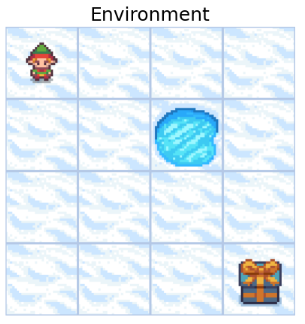
\includegraphics[width=.65\linewidth]{images/Frozen_Lake} \pause
\end{minipage}\begin{minipage}{.5\linewidth}
\centering
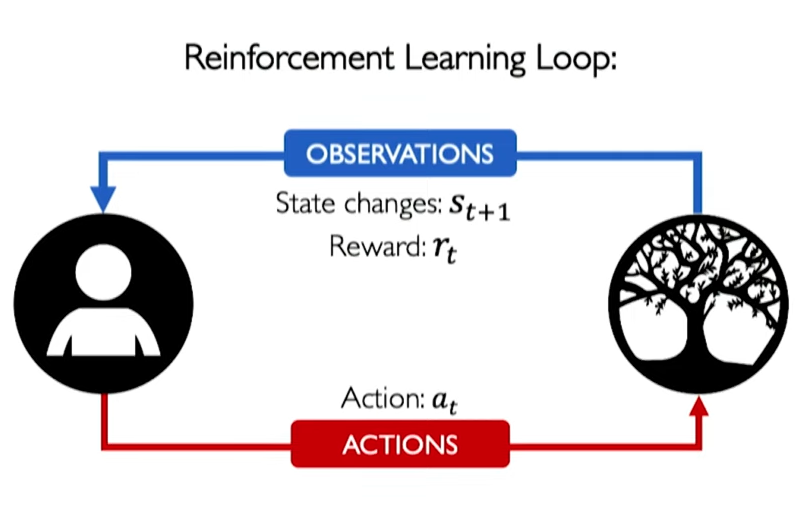
\includegraphics[width=.9\linewidth]{images/RL_loop}
\end{minipage}

\vspace{.5\baselineskip}

\HandRight\ The agent must learn to act based on its experience over an extended period of time.

\end{frame}

\begin{frame}{Components of Reinforcement Learning}

\begin{minipage}{.45\linewidth}

\only<1>{
\begin{itemize}
\item Learning rule
\item Explore vs.~Exploit
\item Long-term reward
\end{itemize}
}
\only<2>{
\begin{itemize}
\item Learning rule
\item {\color{black!30}Explore vs.~Exploit}
\item {\color{black!30}Long-term reward}
\end{itemize}
}
\only<3>{
\begin{itemize}
\item {\color{black!30}Learning rule}
\item Explore vs.~Exploit
\item {\color{black!30}Long-term reward}
\end{itemize}
}
\only<4>{
\begin{itemize}
\item {\color{black!30}Learning rule}
\item {\color{black!30}Explore vs.~Exploit}
\item Long-term reward
\end{itemize}
}

\end{minipage}\hspace{.09\linewidth}\begin{minipage}{.45\linewidth}

\only<2>{
Learning as a correction of the utility estimator’s error based on experience.
}

\only<3>{
Balancing between exploiting current information and exploring to gather better information.
}

\only<4>{
The agent must learn to maximize the total reward of the episode, not just the reward for the current action.
}

\end{minipage}

\end{frame}



%%%%%%%%%%%%%%%%%%%%%%%%%%%%%%%%%%%%%%%%%%
% LEARNING RULE
%%%%%%%%%%%%%%%%%%%%%%%%%%%%%%%%%%%%%%%%%%
\section{Learning Rule}

\begin{frame}{Estimation}

Each round, we want to estimate a natural number $q$ based on imperfect observations $G_1, \ldots, G_T$, where $G_i$ is the observation obtained in the $i$-th round. Suppose $Q$ is our current estimate.

\pause

\vspace{.5\baselineskip}

\begin{center}

\begin{tikzpicture}
\draw (-4,1) -- (4, 1);
\only<2->{
\node (1) at (0,1) {};
\node (G1) at (0,0) {$G_1$};
\draw[arrow] (G1) -- (1);
}
\only<3-4>{
\node (Q) at (0,1) {};
\node (q) at (0,2) {$Q$};
\draw[arrowR] (q) -- (Q);
}
\only<4->{
\node (2) at (2,1) {};
\node (G2) at (2,0) {$G_2$};
\draw[arrow] (G2) -- (2);
}
\only<5-6>{
\node (Q) at (1,1) {};
\node (q) at (1,2) {$Q$};
\draw[arrowR] (q) -- (Q);
}
\only<6->{
\node (3) at (-3,1) {};
\node (G3) at (-3,0) {$G_3$};
\draw[arrow] (G3) -- (3);
}
\only<7->{
\node (Q) at (-1.5,1) {};
\node (q) at (-1.5,2) {$Q$};
\draw[arrowR] (q) -- (Q);
}
\end{tikzpicture}

\end{center}

\vspace{-.5\baselineskip}

\only<8>{
What formula can we use to measure the direction and magnitude of the change in the estimate?
}

\end{frame}

\begin{frame}{Error Correction in Estimation}

Each round, we observe a $G_i$ and note the variation with respect to our current estimate $q$.

%\vspace{\baselineskip}

\begin{center}

\begin{tikzpicture}
\draw (-4,1) -- (4, 1);
\node (1) at (0,1) {};
\node (G1) at (0,0) {$G_1$};
\draw[arrow] (G1) -- (1);
\node (2) at (2,1) {};
\node (G2) at (2,0) {$G_2$};
\draw[arrow] (G2) -- (2);
\only<1-2>{
\node (Q) at (0,1) {};
\node (q) at (0,2) {$Q$};
\draw[arrowR] (q) -- (Q);
}
\only<3-4>{
\node (Q) at (1,1) {};
\node (q) at (1,2) {$q$};
\draw[arrowR] (q) -- (Q);
}
\only<4->{
\node (3) at (-3,1) {};
\node (G3) at (-3,0) {$G_3$};
\draw[arrow] (G3) -- (3);
}
\only<5>{
\node (Q) at (-1.5,1) {};
\node (q) at (-1.5,2) {$Q$};
\draw[arrowR] (q) -- (Q);
}
\end{tikzpicture}

\vspace{\baselineskip}

\only<1>{
The estimation error is $\delta = G_2 - Q$.
}
\only<2>{
$G_2$ is not the actual data $q$, so we must weight the error by a learning rate $\alpha$.
}
\only<3>{
We update $Q$ using the rule
%
\[
Q\gets Q + \alpha\delta
\]
}
\only<4>{
The estimation error is $\delta = G_3 - Q$.
}
\only<5>{
\vspace{-2\baselineskip}
\[
Q\gets Q + \alpha\bigl( G_3 - Q \bigr)
\]
}

\end{center}

\end{frame}

\begin{frame}{Multi-armed Bandits}

\begin{minipage}{.65\linewidth}
\begin{center}
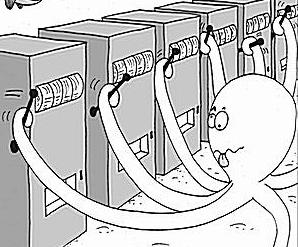
\includegraphics[width=0.6\linewidth]{images/multiarmedbandit}
\end{center}
\end{minipage}\begin{minipage}{.35\linewidth}
Stochastic\par scheduling\par problem
\end{minipage}

\vspace{\baselineskip}

\begin{itemize}
\only<1>{
\item The agent pulls the lever of one of the machines and gets a reward of 0 or 1.
}
\only<2>{
\item The success probability of each machine is different and initially unknown to the agent.
}
\end{itemize}

\end{frame}

\begin{frame}{Multi-armed Bandit Problem}

\vspace{-1\baselineskip}

\begin{center}
\begin{minipage}{.3\linewidth}
\begin{center}
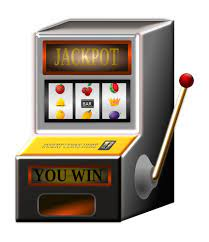
\includegraphics[width=0.9\textwidth]{images/slotmachine}

\
$r(1)$
\end{center}
\end{minipage}\begin{minipage}{.3\linewidth}
\begin{center}
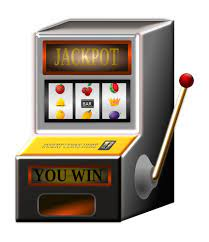
\includegraphics[width=0.9\textwidth]{images/slotmachine}

\
$r(2)$
\end{center}
\end{minipage}
\end{center}

\vspace{.5\baselineskip}

\textbf{Problem:} Which machine $a$ offers success with the highest probability $Q(a)$?

\end{frame}

\begin{frame}{Solution Plan}

\HandRight\ Estimate the success probability $q(a)$ of each machine $a$. \pause

\vspace{\baselineskip}

\HandRight\ Each round $i$, select a machine $a$ and observe the reward $r_i$. \pause

\vspace{\baselineskip}

\HandRight\ Maintain the estimators $Q_i(a)$ and update using the rule:
%
\[
Q_i(a) = \begin{cases}
Q_{i-1}(a) + \alpha\bigl(r_i - Q_{i-1}(a)\bigr), & \text{if $a$ is selected}\cr
Q_{i-1}(a), & \text{otherwise}
\end{cases}
\]

\end{frame}

\begin{frame}{Example}

Suppose $\alpha=\frac{1}{2}$.

\vspace{\baselineskip}

\begin{minipage}{.5\linewidth}
\begin{center}
Machine 1
\end{center}

\begin{itemize}
\item<1-> \textit{Initial state:} $Q_0(1) = 0$
\item<2-> \textit{Round 1:} $Q_1(1) = 0 + \alpha(1 - 0) = \frac{1}{2}$
\item<3-> \textit{Round 2:} $Q_2(1) = \frac{1}{2} + \alpha(0 - \frac{1}{2})= \frac{1}{4}$
\item<4-> \textit{Round 3:} $Q_3(1) = \frac{1}{4}$
\end{itemize}
\end{minipage}\begin{minipage}{.5\linewidth}
\begin{center}
Machine 2
\end{center}

\begin{itemize}
\item<1-> \textit{Initial state:} $Q_0(2) = 0$
\item<2->  \textit{Round 1:} $Q_1(2) = 0$
\item[]
\item<3-> \textit{Round 2:} $Q_2(2) = 0$
\item<4-> \textit{Round 3:} $Q_3(2) = 0 + \alpha(1 - 0) = \frac{1}{2}$
\end{itemize}
\end{minipage}

\vfill

\only<1>{Both estimators start at 0.}
\only<2>{We select 1 and achieve success ($r_1=1$).}
\only<3>{We select 1 and \alert{do not} achieve success ($r_2=0$).}
\only<4>{We select 2 and achieve success ($r_3=1$).}

\vspace{\baselineskip}

\end{frame}



%%%%%%%%%%%%%%%%%%%%%%%%%%%%%%%%%%%%%%%%%%
% EXPLORE VS. EXPLOIT
%%%%%%%%%%%%%%%%%%%%%%%%%%%%%%%%%%%%%%%%%%
\section{Explore vs.~Exploit}

\begin{frame}{Explore vs.~Exploit (1/3)}

Two extreme approaches:

\begin{itemize}
\item \textbf{Explore}: Sample both arms.
\item \textbf{Exploit}: Select the arm that has provided the best rewards so far (greedy strategy).
\end{itemize}

\pause

\begin{minipage}{.6\linewidth}
\begin{center}
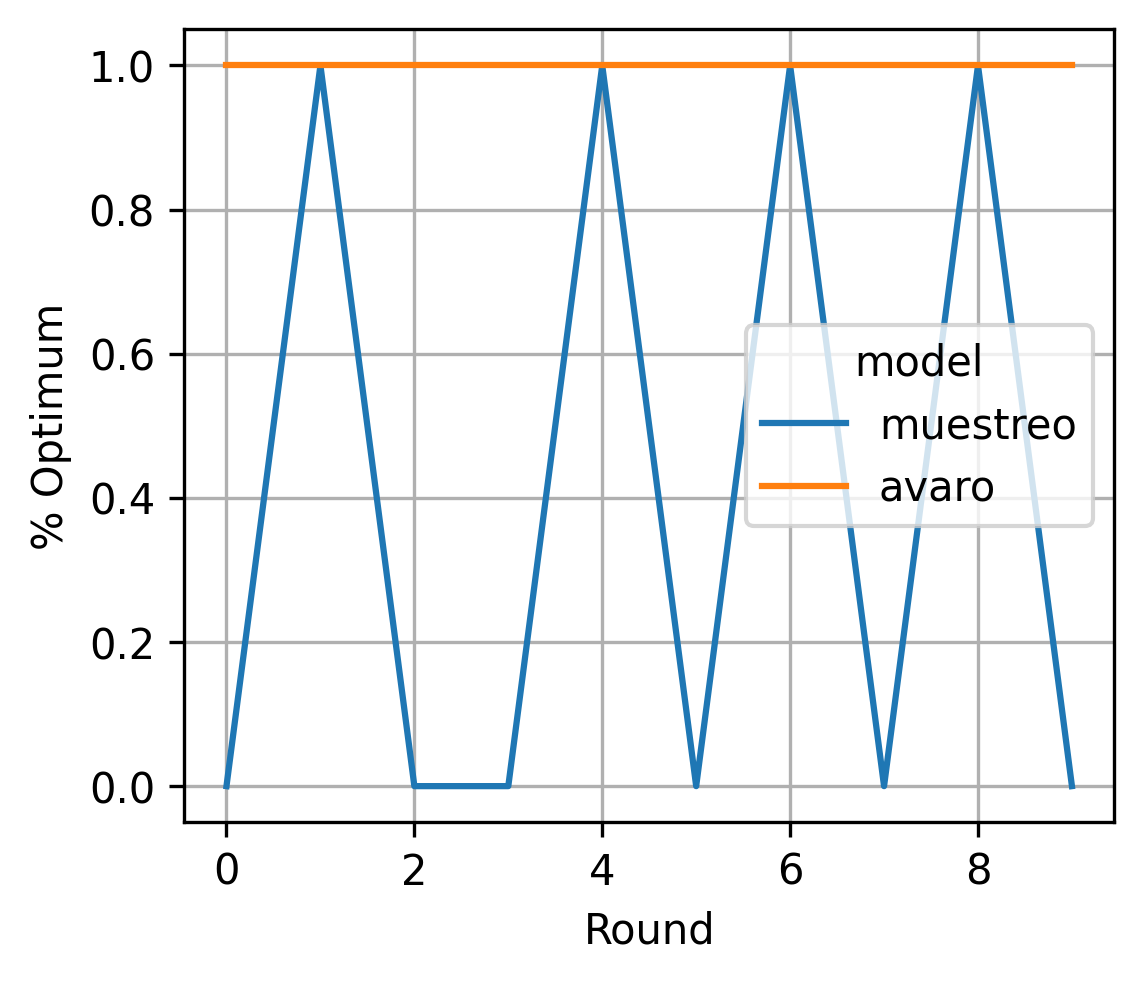
\includegraphics[width=0.8\textwidth]{images/arriba}
\end{center}
\end{minipage}\begin{minipage}{.4\linewidth}
\begin{itemize}
\item The sampling strategy exhibits random behavior.
\item<3-> The greedy strategy tried the optimal arm and succeeded.
\end{itemize}
\end{minipage}

\end{frame}

\begin{frame}{Explore vs.~Exploit (2/3)}

Two extreme approaches:

\begin{itemize}
\item \textbf{Explore}: Sample both arms.
\item \textbf{Exploit}: Select the arm that has provided the best rewards so far (greedy strategy).
\end{itemize}

\begin{minipage}{.6\linewidth}
\begin{center}
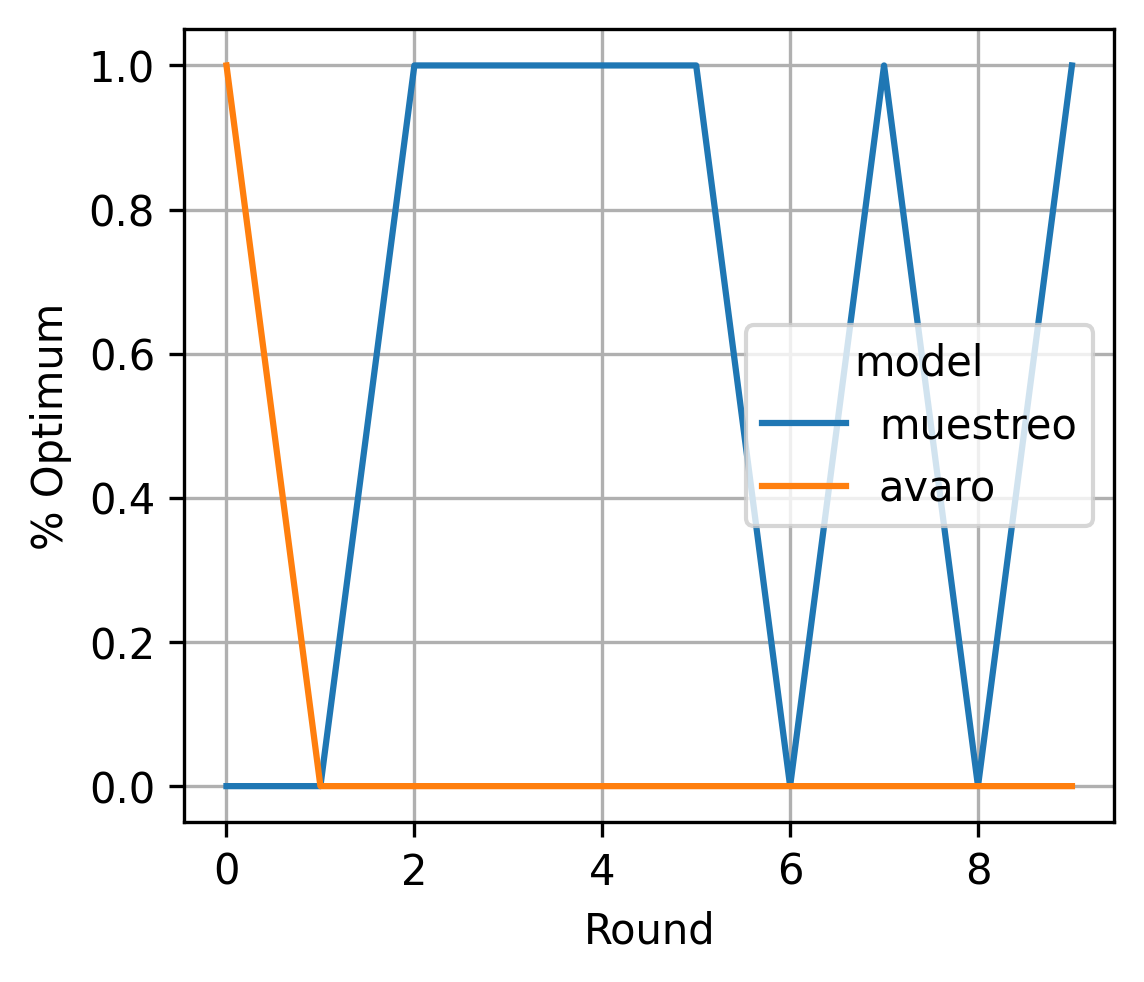
\includegraphics[width=0.8\textwidth]{images/abajo}
\end{center}
\end{minipage}\begin{minipage}{.4\linewidth}
\begin{itemize}
\item The greedy strategy tried the optimal arm without success.
\item Then, the greedy strategy succeeded by trying the arm that is NOT optimal.
\end{itemize}
\end{minipage}

\end{frame}

\begin{frame}{Explore vs.~Exploit (3/3)}

Two extreme approaches:

\begin{itemize}
\item \textbf{Explore}: Sample both arms.
\item \textbf{Exploit}: Select the arm that has provided the best rewards so far (greedy strategy).
\end{itemize}

\begin{minipage}{.6\linewidth}
\begin{center}
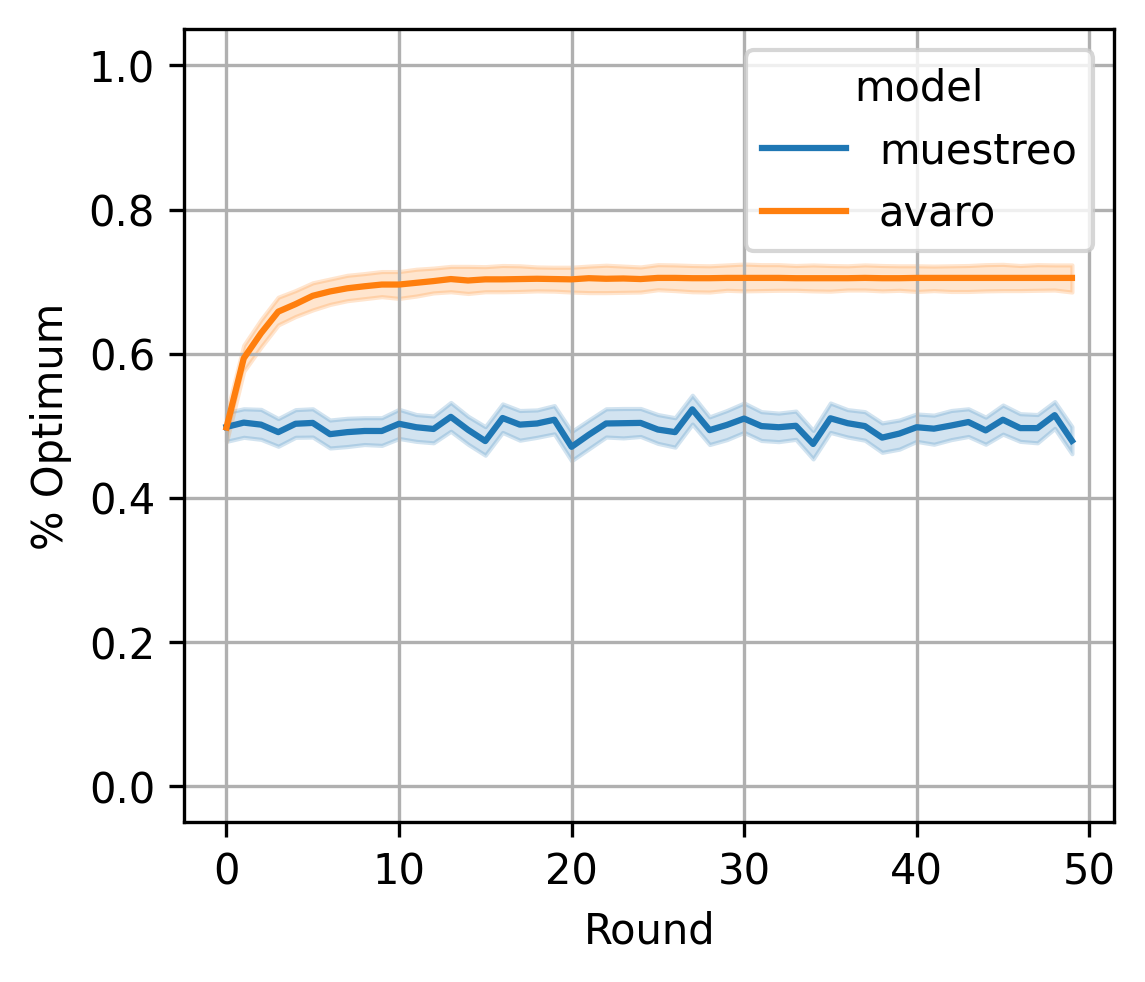
\includegraphics[width=0.8\textwidth]{images/muestreo_vs_explorar}
\end{center}
\end{minipage}\begin{minipage}{.4\linewidth}
Average over 50\par experiments of 50 trials each.
\end{minipage}

\end{frame}

\begin{frame}{Possible Solutions}

There are various ways to address the dilemma between explore and exploit:

\

\begin{itemize}
\item Optimistic initial greedy
\item $\epsilon$-greedy
\item $\epsilon$-greedy with annealing
\item Upper Confidence Bound
\item Softmax
\item Etc.
\end{itemize}

\vspace{\baselineskip}

\HandRight\ Here, we will only discuss the $\epsilon$-greedy strategy.

\end{frame}

\begin{frame}{$\epsilon$-greedy (1/2)}

Balance between exploit (with probability $1-\epsilon$) and explore (with probability $\epsilon$).

\begin{center}
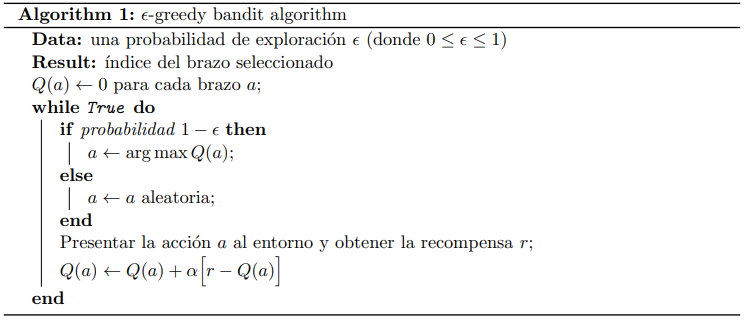
\includegraphics[width=0.85\textwidth]{images/e-greedy}
\end{center}

\end{frame}

\begin{frame}{$\epsilon$-greedy (2/2)}

Results:

\vspace{-\baselineskip}

\begin{center}
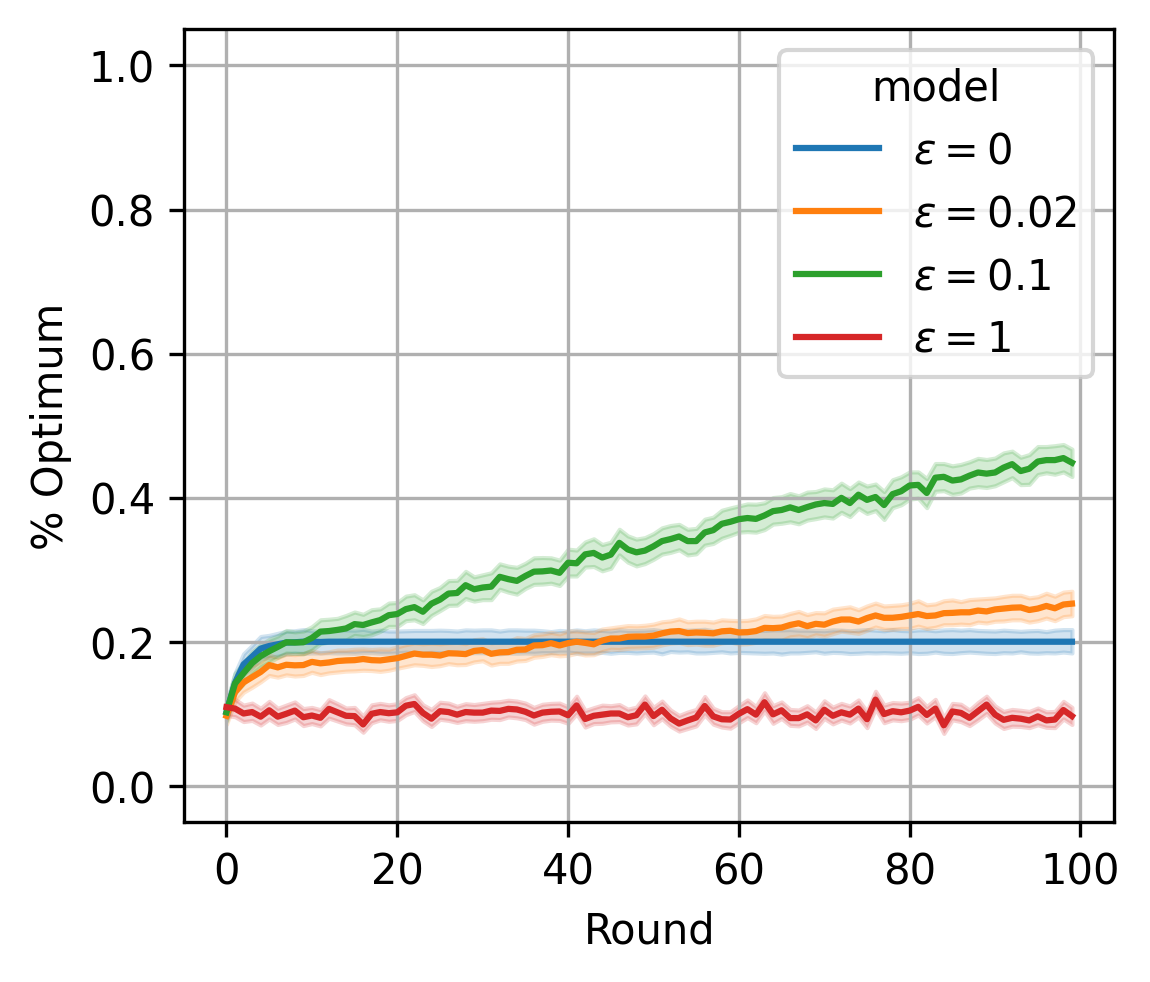
\includegraphics[width=0.5\textwidth]{images/e-greedys}
\end{center}

\vspace{-\baselineskip}

Protocol:

10 arms. 50 experiments of 50 trials.

\end{frame}


%%%%%%%%%%%%%%%%%%%%%%%%%%%%%%%%%%%%%%%%%%
% LONG TERM REWARD
%%%%%%%%%%%%%%%%%%%%%%%%%%%%%%%%%%%%%%%%%%
\section{Long-term Reward}

\begin{frame}{Definitions}

\begin{itemize}
\item<1-> \textbf{Utility}: 

\vspace{-\baselineskip}

\[
G = r_1 + \gamma r_2 + \gamma^2 r_3 + \ldots = \sum_{t=0}^{\infty} \gamma^k r_{t+1}
\]

\item<2-> \textbf{Policy}: A function $\pi$ that for each state $s$ returns a probability distribution over possible actions, such that $\pi(a|s)$ is the probability of taking action $a$ in state $s$.

\item<3-> \textbf{State Value}: The expected utility $v_{\pi}(s)$ of following policy $\pi$ from state $s$: $v_{\pi}(s) = \mathbb{E}[G | s]$.

\item<4-> \textbf{Action Value}: The expected utility of performing an action $a$ in state $s$ and then following $\pi$: $q_{\pi}(s,a) = \mathbb{E}[G | s,a]$
\end{itemize}

\end{frame}

\begin{frame}{Transition Stochasticity}

\begin{minipage}{.3\linewidth}

\includegraphics[width=.95\linewidth]{images/robot}
\end{minipage}\hspace{.05\linewidth}\begin{minipage}{.6\linewidth}

After the agent executes action $a$ in state $s$, it transitions to state $s_i$ with probability $p(s_i | s, a)$.

\begin{center}
\[
\{p(s_1 | s, a); p(s_2 | s, a); \ldots; p(s_n | s, a)\}
\]

\end{center}
\end{minipage}

\end{frame}

\begin{frame}{Markov Property}

\HandRight\ Path Independence

\

\begin{center}
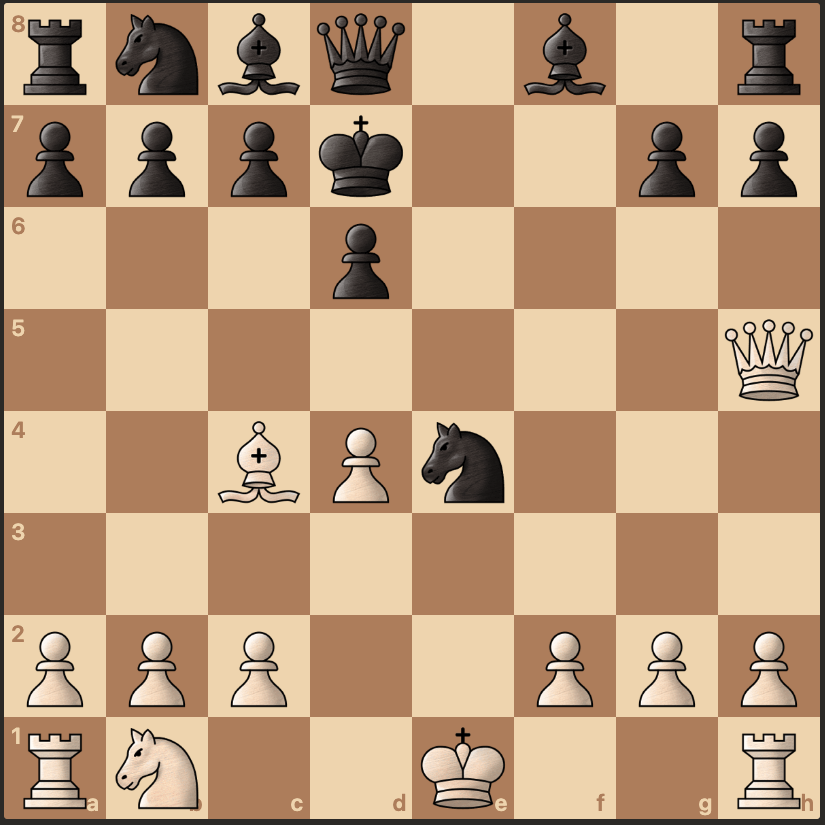
\includegraphics[width=.3\linewidth]{images/ajedrez}
\end{center}

\[
p(s_{t+1} | s_0, a_0, s_1, a_1, \ldots, s_t, a_t) = p(s_{t+1} | s_t, a_t)
\]

\end{frame}


\begin{frame}{Components of MDPs}

\begin{minipage}{.5\linewidth}
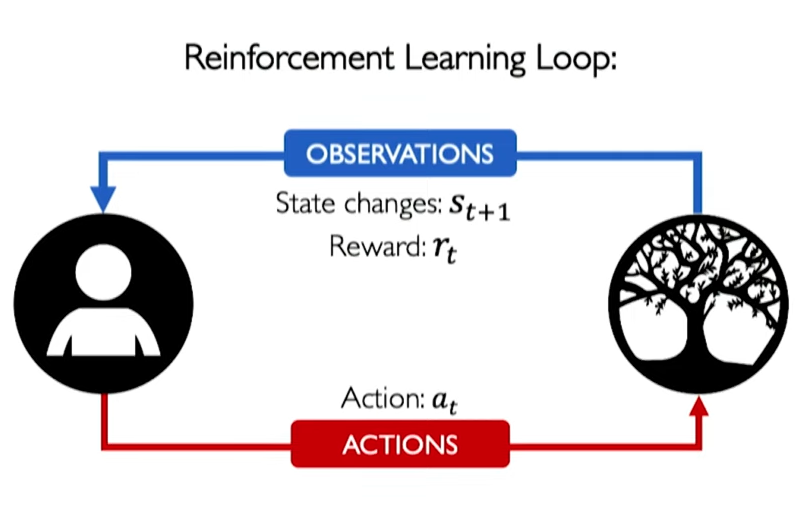
\includegraphics[width=.9\linewidth]{images/RL_loop}
\end{minipage}\begin{minipage}{.5\linewidth}
\begin{itemize}
\item Set of states
\item Subset of terminal states
\item Set of actions
\item \only<1-2>{Transitions $p(s' | s,a)$}\only<3->{\sout{Transitions $p(s' | s,a)$}}
\item \only<1-2>{Rewards $r(s,a,s')$}\only<3->{\sout{Rewards $r(s,a,s')$}}
\end{itemize}
\end{minipage}

\vspace{\baselineskip}

\only<2>{
\[
v_{\pi}(s) = \sum_a\pi(a|s)\sum_{s'}\left( p(s' | s,a) \Bigl[ r(s,a,s') + \gamma v_{\pi}(s') \Bigr] \right)
\]
}

\visible<3->{
\only<3>{
\HandRight\ Let us assume that we do not know the MDP model.  
}
\only<4>{
\HandRight\ We aim to estimate $v_{*}$ and $q_{*}$ directly.  
}
} % end visible

\end{frame}


%%%%%%%%%%%%%%%%%%%%%%%%%%%%%%%%%%%%%%%%%%
% TEMPORAL DIFFERENCE METHODS
%%%%%%%%%%%%%%%%%%%%%%%%%%%%%%%%%%%%%%%%%%
\section{Temporal Difference Methods}

\begin{frame}{Using the Bellman Equation}

\begin{minipage}{.5\linewidth}
\textbf{Dynamic Programming:}

\scalebox{.6}{
\begin{minipage}{\linewidth}
\[
V_{k+1}(s) \gets \sum_a\pi(a|s)\sum_{s'}\left( p(s' | s,a) \Bigl[ r + \gamma V_k(s') \Bigr] \right)
\]
\end{minipage}
} % end scalebox

\begin{center}
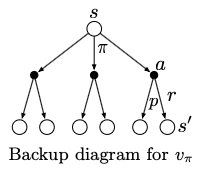
\includegraphics[width=.45\linewidth]{images/backup_diagram_v}
\end{center}

\end{minipage}\begin{minipage}{.5\linewidth}

\textbf{Temporal Difference:}

\scalebox{.8}{
\begin{minipage}{\linewidth}
\only<2>{
\[
V_{k+1}(s) \gets V_k(s) + \alpha\left( \alert{G} - V_k(s) \right)
\]
}
\only<3>{
\[
V_{k+1}(s) \gets V_k(s) + \alpha\left( \alert{r + \gamma V_k(s')} - V_k(s) \right)
\]
}
\end{minipage}
} % end scalebox

\begin{center}
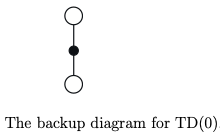
\includegraphics[width=.5\linewidth]{images/backup_td}
\end{center}

\only<1>{\vspace{1.5\baselineskip}}
\only<2->{\vspace{.5\baselineskip}}

\end{minipage}

\end{frame}

\begin{frame}{Learning Rule}

\[
V(s) \gets \overbrace{V(s)}^{\txt{previous\\estimate}} + \underbrace{\alpha}_{\txt{step\\size}}\Bigl(\overbrace{r_1 + \gamma \underbrace{V(s_1)}_{bootstrap}}^{\txt{new\\data}} - \underbrace{V(s)}_{\txt{previous\\estimate}}\Bigr)
\]

\end{frame}

\begin{frame}{Learning a Policy (SARSA)}

Suppose a policy $\pi$.

\vspace{.5\baselineskip}

\begin{itemize}
\item<2-> Rule to update state-action values:
%
\[
Q(s,a) \gets Q(s,a) + \alpha\Bigl(r + \gamma Q(s',a') - Q(s,a)\Bigr)
\]
%
\item[]<2-> Where $s'$ is the state reached after performing $a$ in $s$,
\item[]<2-> and $a'\gets$ action by sampling $\pi(s')$.

\item<3-> Improve $\pi(s)$ with $\epsilon$-greedy using $Q$ for all $s$.

\end{itemize}

\end{frame}

\begin{frame}{The $Q$ Table}

Consider the ABC environment presented two classes ago.

\vspace{\baselineskip}

\begin{minipage}{.5\linewidth}

\begin{center}
\begin{tikzpicture}
\draw (0,0) rectangle (.5,.5);
\draw (0.5,0) rectangle (1,.5);
\draw (1,0) rectangle (1.5,.5);
\node (A) at (0.25, 0.25) {$A$};
\node (B) at (0.75, 0.25) {$B$};
\node (C) at (1.25, 0.25) {$C$};
\only<1-8>{
\node (ag) at (0.25,-1) {
\includegraphics[width=.75cm]{images/agent}};
\draw[arrow] (ag) -- (A);
}
\only<9->{
\node (ag) at (0.75,-1) {
\includegraphics[width=.75cm]{images/agent}};
\draw[arrow] (ag) -- (B);
}
\end{tikzpicture}
\end{center}

\end{minipage}\begin{minipage}{.5\linewidth}

\begin{center}
\begin{tabular}{ccc}\toprule
       & Left & Right \\
$A$ & \only<1-6>{0}\only<7->{-0.1} & \only<1-11>{0}\only<12->{-0.1} \\
$B$ & 0 & \only<1-15>{0}\only<16->{1} \\
$C$ & 0 & 0 \\\bottomrule
\end{tabular}
\end{center}

\end{minipage}

\vspace{\baselineskip}

\begin{minipage}{.6\linewidth}
\only<2>{
Randomly, the agent selects the\par action Left.
}
\only<3-4>{
The agent remains in state $A$.
}
\only<5>{
\scalebox{.7}{
\begin{minipage}{\linewidth}
$q(A,\text{Left}) += \alpha\Bigl(-1 + \gamma q(A,\text{Right}) - q(A,\text{Left})\Bigr)$
\end{minipage}
}
}
\only<6>{
\scalebox{.7}{
\begin{minipage}{\linewidth}
$q(A,\text{Left}) += 0.1\Bigl(-1 + 0.8\times 0 - 0\Bigr)$
\end{minipage}
}
}
\only<8>{
The agent selects the action with the highest\par $q$ value, namely, Right (this occurs with probability $1-\epsilon$).
}
\only<9>{
Suppose the agent reaches $B$\par (this occurs with probability 0.9).
}
\only<10>{
\scalebox{.65}{
\begin{minipage}{\linewidth}
$q(A,\text{Right})\,{+=}\, \alpha\Bigl(-1 {+} \gamma q(B,\text{Right}) {-} q(A,\text{Right})\Bigr)$
\end{minipage}
}
}
\only<11>{
\scalebox{.65}{
\begin{minipage}{\linewidth}
$q(A,\text{Right})\,{+=}\, 0.1\Bigl(-1 + 0.8\times 0 - 0\Bigr)$
\end{minipage}
}
}
\only<12>{
Randomly, the agent selects the\par action Right.
}
\only<13>{
The agent reaches $C$.
}
\only<14>{
\scalebox{.65}{
\begin{minipage}{\linewidth}
$q(B,\text{Right})\,{+=}\, \alpha\Bigl(10 {+} \gamma q(C,\text{Right}) {-} q(B,\text{Right})\Bigr)$
\end{minipage}
}
}
\only<15>{
\scalebox{.65}{
\begin{minipage}{\linewidth}
$q(B,\text{Right})\,{+=}\, 0.1\Bigl(10 + 0.8\times 0 - 0\Bigr)$
\end{minipage}
}
}
\end{minipage}\begin{minipage}{.4\linewidth}
\begin{center}
\only<3>{
$s=A$

$a=\text{Left}$

$s'=A$

$a'\gets \text{random action}$
}
\only<4>{
$s=A$

$a=\text{Left}$

$s'=A$

$a'\gets \text{Right}$
}
\only<6>{
Suppose $\alpha=0.1$
}
\only<9>{
$s=A$

$a=\text{Right}$

$s'=B$

$a'\gets \text{Right}$
}
\only<12>{
$s=B$

$a=\text{Right}$

$s'=C$

$a'\gets \text{Right}$
}
\end{center}
\end{minipage}

\end{frame}

\begin{frame}{SARSA Pseudocode}

\begin{center}
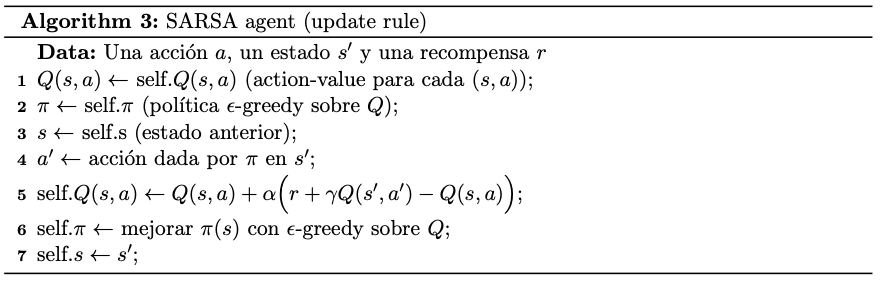
\includegraphics[width=.95\linewidth]{images/sarsa_agent}
\end{center}

\end{frame}

\begin{frame}{SARSA vs. Q-learning (1/2)}

\textbf{SARSA:}

\[
Q(s,a) \gets Q(s,a) + \alpha\Bigl(r + \gamma Q(s',a') - Q(s,a)\Bigr)
\]
\[
\mbox{Improve $\pi(s)$ with $\epsilon$-greedy and $Q$}
\]

\

\textbf{Q-learning:}

\[
Q(s,a) \gets Q(s,a) + \alpha\Bigl(r + \gamma \alert{\max_{a'}Q(s',a')} - Q(s,a)\Bigr)
\]
\[
\mbox{Improve $\pi(s)$ with $\epsilon$-greedy and $Q$}
\]

\end{frame}

\begin{frame}{SARSA vs. Q-learning (2/2)}

\vspace{.5\baselineskip}

\begin{center}
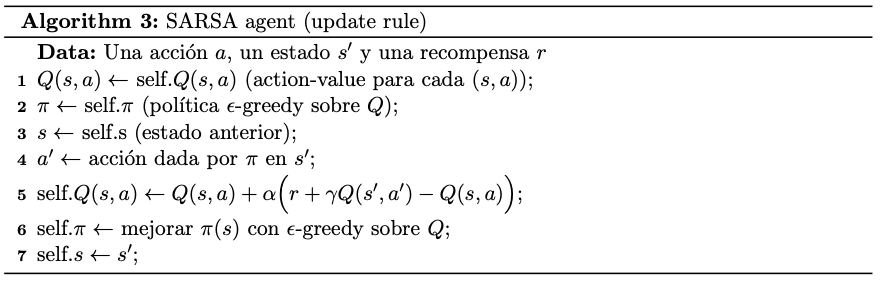
\includegraphics[width=.85\linewidth]{images/sarsa_agent}
\end{center}

\vfill

\begin{center}
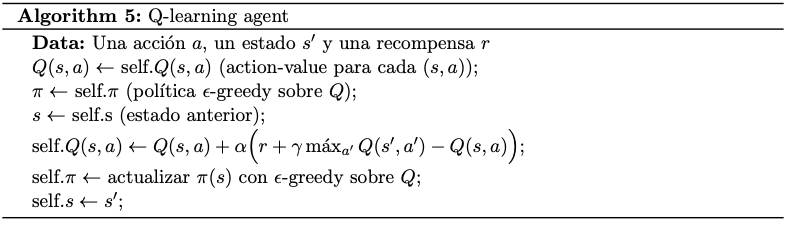
\includegraphics[width=.85\linewidth]{images/q_learning_agent}
\end{center}

\vspace{.5\baselineskip}

\end{frame}

\begin{frame}{The Cliff Problem}

\begin{center}
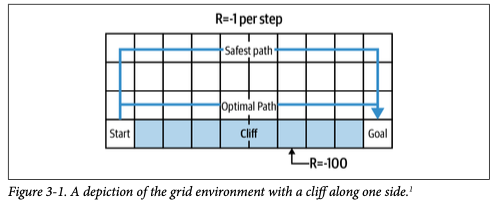
\includegraphics[width=.65\linewidth]{images/Cliff_problem}
\end{center}

\end{frame}

\begin{frame}{Optimal Policy --- SARSA vs. Q-learning}

\begin{minipage}{.6\linewidth}
\begin{center}
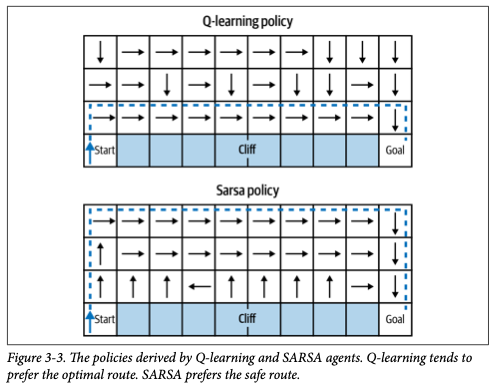
\includegraphics[width=.9\linewidth]{images/Optimal_sarsa_vs_q_learning}
\end{center}
\end{minipage}\begin{minipage}{.4\linewidth}
\begin{center}
$Q$ Table
\end{center}

\vspace{-1.5\baselineskip}

\begin{center}
\scalebox{.6}{
\begin{tabular}{ccccc}\toprule
     & Left & Right & Up & Down \\
20 &       -11        &       -10      &    -11     &   -100     \\
21 &       -10        &       -9       &    -10     &   -100     \\\bottomrule
\end{tabular}
} % end scalebox
\end{center}

\vspace{.5\baselineskip}

\begin{small}
What is the updated value of 

\vspace{-1.5\baselineskip}

\[
q(20, \text{Right})
\]

\vspace{.25\baselineskip}

if $a' = \text{Down}$, using:

\vspace{.25\baselineskip}

\begin{itemize}
\item SARSA?
\item Q-learning?
\end{itemize}
\end{small}

\end{minipage}

\end{frame}

\begin{frame}{Utility --- SARSA vs. Q-learning}

\begin{center}
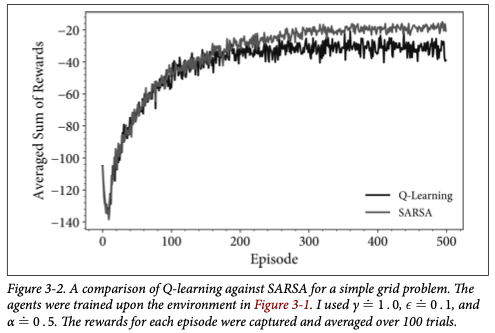
\includegraphics[width=.65\linewidth]{images/utilities_sarsa_vs_q_learning}
\end{center}

\end{frame}




%%%%%%%%%%%%%%%%%%%%%%%%%%%%%%%%%%%%%%%%%%
% TAKE AWAY
%%%%%%%%%%%%%%%%%%%%%%%%%%%%%%%%%%%%%%%%%%
\begin{frame}{Takeaway}

In this session, you learned:

\begin{itemize}
\item To analyze reinforcement learning as the combination of estimating long-term reward, correcting estimation error, and balancing exploit vs. explore.
\item The temporal difference methods SARSA and Q-learning.
\end{itemize}

\end{frame}

\end{document}

